\section{累次积分}
\label{sec:integ-iterated}

计算平面区域上的累计时，我们习惯先沿一个方向积分，再沿另一个方向积分；计算双重级数时，先按行求和再把行和相加。这些做法都把一个联合累计拆成依次累计，并默认两种次序给出同一个结果。

有限矩阵的元素求和可以先行后列，也可以先列后行，这是有限加法的交换律。无穷的情形则需要条件，本节后面会给出一个无穷矩阵，两种次序的结果不同。下面先为两个测度空间的乘积建立集合族和乘积测度，再分别对非负函数与绝对可积函数证明这种拆分与换序成立。

\subsection{乘积测度}
\label{sec:integ-product-measure}

\paragraph{可测矩形与乘积$\sigma$代数}
设$(X,\mathcal A,\mu)$与$(Y,\mathcal B,\nu)$是测度空间。在$X\times Y$上，最简单的集合是$A\times B$，其中$A\in\mathcal A$、$B\in\mathcal B$，称为\term{可测矩形}（measurable rectangle）。它的“面积”应当是$\mu(A)\nu(B)$。可测矩形的有限并一般不再是矩形，所以要像上一章那样由它们生成$\sigma$代数。

\begin{definition}[乘积$\sigma$代数]
\label{def:integ-product-sigma}
由全体可测矩形生成的$\sigma$代数称为\term{乘积$\sigma$代数}（product sigma-algebra），记作$\mathcal A\otimes\mathcal B$。
\end{definition}

可测矩形的“边”可以是任意可测集，不必是区间。图~\ref{fig:integ-product-rectangles}(a)中$A$由两段组成，$A\times B$也就由两块组成，面积仍是$\lambda(A)\lambda(B)=1.8\times1=1.8$。

两个可测矩形之交仍是可测矩形：
\[
 (A\times B)\cap(A'\times B')=(A\cap A')\times(B\cap B').
\]
所以可测矩形构成$\pi$系统，后面的唯一性论证要用到这一点。

\begin{BookInlineFigure}
  \centering
  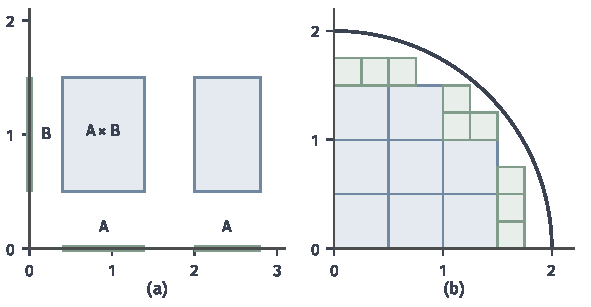
\includegraphics[width=100mm]{figures/04-spaces-measures-and-geometry/02-measure/matplotlib/integ-product-rectangles/figure.pdf}
  \caption{乘积可测结构由矩形生成。(a)取$A=[0.4,1.4]\cup[2.0,2.8]$、$B=[0.5,1.5]$，可测矩形$A\times B$由两块组成，绿色线段分别是$A$与$B$。(b)半径为$2$的四分之一圆盘不是矩形，蓝色矩形是边长$0.5$的网格中完全落在圆盘内的方格，绿色矩形是边长$0.25$的网格补充的方格；逐层加细的矩形不交并从内部逼近圆盘。}
  \label{fig:integ-product-rectangles}
\end{BookInlineFigure}

在欧氏空间上，乘积$\sigma$代数就是Borel代数：
\begin{equation}
 \mathcal B(\mathbb R)\otimes\mathcal B(\mathbb R)=\mathcal B(\mathbb R^2).
 \label{eq:integ-borel-product}
\end{equation}
一方面，开集是可数个有理顶点开矩形之并，开矩形是可测矩形，如图~\ref{fig:integ-product-rectangles}(b)所示，所以Borel集都在乘积$\sigma$代数中。另一方面，$A\times\mathbb R$是$A$在连续投影下的原像，对Borel集$A$是Borel集；$A\times B$是这样两个集合之交，也是Borel集。

\paragraph{截面}
依次累计的第一步是固定一个坐标。对$E\subseteq X\times Y$与$x\in X$，称$E_x=\{y\in Y:(x,y)\in E\}$为$E$在$x$处的\term{截面}（section）；类似地，$E^y=\{x\in X:(x,y)\in E\}$。对函数$f$，固定$x$得到截面函数$f_x(y)=f(x,y)$，固定$y$得到$f^y(x)=f(x,y)$。

截面的形状取决于固定哪个坐标。圆环在靠近中心的$x$处的截面是两段区间，在靠外的$x$处则是一段。下面先确认截面总是可测的，否则内层积分无从谈起。

\begin{lemma}[截面的可测性]
\label{lem:integ-section-measurable}
若$E\in\mathcal A\otimes\mathcal B$，则对每个$x$有$E_x\in\mathcal B$，对每个$y$有$E^y\in\mathcal A$。若$f$是$\mathcal A\otimes\mathcal B$可测函数，则每个$f_x$是$\mathcal B$可测的，每个$f^y$是$\mathcal A$可测的。
\end{lemma}

\begin{proof}
固定$x$，令$\mathcal E$为满足$E_x\in\mathcal B$的集合$E\subseteq X\times Y$全体。截面与补集、可数并可交换：
\[
 (X\times Y\setminus E)_x=Y\setminus E_x,\qquad\Bigl(\bigcup_nE_n\Bigr)_x=\bigcup_n(E_n)_x .
\]
所以$\mathcal E$是$\sigma$代数。对可测矩形，$(A\times B)_x$在$x\in A$时为$B$、否则为空集，所以$\mathcal E$含全部可测矩形，从而含$\mathcal A\otimes\mathcal B$。函数的情形由$\{f_x>a\}=(\{f>a\})_x$得到。$y$一侧对称。
\end{proof}

\paragraph{截面测度的可测性}
乘积测度的候选定义是沿$x$累计截面的测度，这相当于把区域切成薄片，每片的“长度”乘以厚度再相加：
\[
 E\mapsto\int_X\nu(E_x)\,\mathrm d\mu(x).
\]
为此要先知道$x\mapsto\nu(E_x)$可测。这一步需要$\sigma$有限条件。

\begin{lemma}[截面测度的可测性]
\label{lem:integ-section-measure}
设$\nu$是$\sigma$有限测度，$E\in\mathcal A\otimes\mathcal B$。则$x\mapsto\nu(E_x)$是$X$上的可测函数。
\end{lemma}

\begin{proof}
先设$\nu$有限。令$\mathcal D$为使$x\mapsto\nu(E_x)$可测的$E\in\mathcal A\otimes\mathcal B$全体。对可测矩形，$\nu((A\times B)_x)=\nu(B)\mathbf 1_A(x)$，可测，所以$\mathcal D$含可测矩形这一$\pi$系统。

$\mathcal D$是$\lambda$系统，逐条核对。全集$X\times Y$的截面测度是常数$\nu(Y)$。补集的截面测度为$\nu(Y)-\nu(E_x)$，这里用到$\nu$有限，差才有意义。不交可数并的截面测度是各截面测度之和，可测函数的可数和可测。由$\pi$--$\lambda$定理，$\mathcal D=\mathcal A\otimes\mathcal B$。

一般情形取$Y_m\in\mathcal B$两两不交、并为$Y$且$\nu(Y_m)<+\infty$，令$\nu_m(B)=\nu(B\cap Y_m)$。每个$\nu_m$有限，由上一段$x\mapsto\nu_m(E_x)$可测，而$\nu(E_x)=\sum_m\nu_m(E_x)$是可数个可测函数之和。
\end{proof}

\paragraph{乘积测度的构造}
截面测度可测以后，沿$x$累计截面测度就得到一个候选的乘积测度；沿$y$累计得到另一个候选。下面的定理说明二者是同一个测度，并且它由矩形上的取值唯一确定。

\begin{theorem}[乘积测度的存在唯一性]
\label{thm:integ-product-measure}
设$\mu,\nu$都是$\sigma$有限测度。则$\mathcal A\otimes\mathcal B$上存在唯一的测度$\pi$，使
\begin{equation}
 \pi(A\times B)=\mu(A)\nu(B),\qquad A\in\mathcal A,\ B\in\mathcal B,
 \label{eq:integ-product-rectangle}
\end{equation}
并且对每个$E\in\mathcal A\otimes\mathcal B$，
\begin{equation}
 \pi(E)=\int_X\nu(E_x)\,\mathrm d\mu(x)=\int_Y\mu(E^y)\,\mathrm d\nu(y).
 \label{eq:integ-product-sections}
\end{equation}
\end{theorem}

\begin{proof}
令$\pi_1(E)=\int_X\nu(E_x)\,\mathrm d\mu(x)$，由引理~\ref{lem:integ-section-measure}，被积函数非负可测。空集的截面都是空集，所以$\pi_1(\varnothing)=0$。若$E_n$两两不交，各截面$(E_n)_x$也两两不交，于是$\nu((\bigcup_nE_n)_x)=\sum_n\nu((E_n)_x)$。对$x$积分并用式~\eqref{eq:integ-series-termwise}逐项积分，得到
\[
 \pi_1\Bigl(\bigcup_nE_n\Bigr)=\sum_n\pi_1(E_n).
\]
所以$\pi_1$是测度。对矩形，
\[
 \pi_1(A\times B)=\int_X\nu(B)\mathbf 1_A\,\mathrm d\mu=\mu(A)\nu(B).
\]
同理$\pi_2(E)=\int_Y\mu(E^y)\,\mathrm d\nu(y)$也是满足式~\eqref{eq:integ-product-rectangle}的测度。

唯一性。取$X_n\in\mathcal A$、$Y_m\in\mathcal B$分别覆盖$X$、$Y$且测度有限，可数个矩形$X_n\times Y_m$覆盖$X\times Y$，在任何满足式~\eqref{eq:integ-product-rectangle}的测度下都取有限值。两个这样的测度在可测矩形这一$\pi$系统上相等，由第~\ref{chap:measure}章生成$\pi$系统上的唯一性定理，它们在$\mathcal A\otimes\mathcal B$上相等。特别地$\pi_1=\pi_2$，这就是式~\eqref{eq:integ-product-sections}。
\end{proof}

\begin{definition}[乘积测度]
\label{def:integ-product-measure}
定理~\ref{thm:integ-product-measure}中的测度称为$\mu$与$\nu$的\term{乘积测度}（product measure），记作$\mu\otimes\nu$。
\end{definition}

下面在一个可以逐项计算的网格上验证式~\eqref{eq:integ-product-sections}。两种切法分别相当于先按行、先按列累计，结果相同正是这个公式的含义。

\begin{example}[有限网格上的乘积测度]
\label{ex:integ-product-grid}
取$X=\{1,2\}$，质量为$\mu(\{1\})=1$、$\mu(\{2\})=2$；取$Y=\{a,b,c\}$，质量为$\nu(\{a\})=1$、$\nu(\{b\})=3$、$\nu(\{c\})=1$。乘积测度给格点$(i,y)$的质量$\mu(\{i\})\nu(\{y\})$。取
\[
 E=\{(1,a),(1,b),(2,b),(2,c)\}.
\]
按$x$切，两个截面的$\nu$测度为
\[
 \nu(E_1)=1+3=4,\qquad\nu(E_2)=3+1=4,
\]
于是
\[
 \int\nu(E_x)\,\mathrm d\mu=1\cdot4+2\cdot4=12 .
\]

按$y$切，三个截面的$\mu$测度为
\[
 \mu(E^a)=1,\qquad\mu(E^b)=1+2=3,\qquad\mu(E^c)=2,
\]
于是
\[
 \int\mu(E^y)\,\mathrm d\nu=1\cdot1+3\cdot3+1\cdot2=12 .
\]
两种切法得到同一个数。
\end{example}

\paragraph{与Lebesgue测度的关系}
在$\mathbb R^2$上，$\lambda\otimes\lambda$与第~\ref{chap:measure}章的二维Lebesgue测度$\lambda_2$都定义在式~\eqref{eq:integ-borel-product}的$\sigma$代数上，在左开右闭矩形上都等于边长之积；由唯一性它们相等。归纳可得$\lambda_d$等于$d$个$\lambda$的乘积。于是$\mathbb R^d$上Borel函数的积分可以逐个坐标计算，这是下面两个定理的主要用途。

\paragraph{乘积集合族与完备化}
乘积$\sigma$代数与测度的完备化是两回事。即使$\mu,\nu$都完备，$\mathcal A\otimes\mathcal B$也未必完备。取$\mathcal L$为Lebesgue可测集，$S\subseteq\mathbb R$不Lebesgue可测，$E=S\times\{0\}$。$E$含于$\mathbb R\times\{0\}$，后者的$\lambda\otimes\lambda$测度为$0$，所以$E$属于完备化；但截面$E^0=S$不可测，由引理~\ref{lem:integ-section-measurable}，$E\notin\mathcal L\otimes\mathcal L$。

二维Lebesgue可测集是$\lambda_2$的完备化，它比$\mathcal L\otimes\mathcal L$大。所以在完备化的乘积测度下，不能默认每个截面都可测；下面的定理会把这种例外限制在零测的参数集上。

\subsection{Tonelli定理}
\label{sec:integ-tonelli}

\paragraph{非负函数的换序}
式~\eqref{eq:integ-product-sections}说的是指示函数的联合积分等于两种次序的累次积分。对一般的非负函数，沿积分的构造步骤推广：指示函数、简单函数、递增极限。非负贡献不会相互抵消，所以结论允许各方都等于$+\infty$。先对一个变量积分、再对另一个变量积分所得的量称为\term{累次积分}（iterated integral）。

\begin{theorem}[Tonelli定理]
\label{thm:integ-tonelli}
设$\mu,\nu$都是$\sigma$有限测度，$f:X\times Y\to[0,+\infty]$是$\mathcal A\otimes\mathcal B$可测函数。则$x\mapsto\int_Yf_x\,\mathrm d\nu$与$y\mapsto\int_Xf^y\,\mathrm d\mu$分别可测，并且下面三者在$[0,+\infty]$中相等：
\begin{equation}
\begin{aligned}
 \int_{X\times Y}f\,\mathrm d(\mu\otimes\nu)&=\int_X\Bigl(\int_Yf(x,y)\,\mathrm d\nu(y)\Bigr)\mathrm d\mu(x)\\
 &=\int_Y\Bigl(\int_Xf(x,y)\,\mathrm d\mu(x)\Bigr)\mathrm d\nu(y).
\end{aligned}
 \label{eq:integ-tonelli}
\end{equation}
\end{theorem}

\begin{proof}
由引理~\ref{lem:integ-section-measurable}，各截面函数可测，内层积分有意义。证明按函数的构造分三步，只写$x$先固定的一侧，另一侧对称。

第一步，$f=\mathbf 1_E$，$E\in\mathcal A\otimes\mathcal B$。内层积分是$\nu(E_x)$，由引理~\ref{lem:integ-section-measure}可测，外层积分等于$(\mu\otimes\nu)(E)$，这就是式~\eqref{eq:integ-product-sections}。

第二步，$f$是非负简单函数，即有限个$c_i\mathbf 1_{E_i}$之和。内层积分是相应$c_i\nu((E_i)_x)$之和，可测，由线性性逐项得到式~\eqref{eq:integ-tonelli}。

第三步，一般的$f$。取二进分层逼近$\varphi_n\uparrow f$，每个$\varphi_n$是$\mathcal A\otimes\mathcal B$可测的简单函数。对每个$x$，$(\varphi_n)_x\uparrow f_x$，由单调收敛定理，
\[
 \int_Y(\varphi_n)_x\,\mathrm d\nu\uparrow\int_Yf_x\,\mathrm d\nu .
\]
作为可测函数的递增极限，$x\mapsto\int f_x\,\mathrm d\nu$可测。再对$x$用一次单调收敛定理，并在乘积空间上对$\varphi_n\uparrow f$用一次，由第二步的等式取极限即得。
\end{proof}

换序的实际用处是：内层积分按一种次序算不出来，换一种次序就能算。下面的例子中，$e^{y^2}$没有初等原函数，先对$y$积分行不通，先对$x$积分却只是乘以区间长度。

\begin{example}[换序计算]
\label{ex:integ-tonelli-swap}
计算累次积分
\[
 I=\int_0^1\Bigl(\int_x^1e^{y^2}\,\mathrm dy\Bigr)\mathrm dx .
\]
被积函数$f(x,y)=e^{y^2}\mathbf 1_{\{0\leq x\leq y\leq1\}}$非负且Borel可测，由Tonelli定理可以换序。固定$y$，$x$的截面是$[0,y]$，于是
\[
 I=\int_0^1\Bigl(\int_0^ye^{y^2}\,\mathrm dx\Bigr)\mathrm dy=\int_0^1ye^{y^2}\,\mathrm dy .
\]
令$w=y^2$，$\mathrm dw=2y\,\mathrm dy$，得到
\[
 I=\frac12\int_0^1e^w\,\mathrm dw=\frac{e-1}2 .
\]
换序之所以合法，只因为被积函数非负，不需要事先知道积分有限。
\end{example}

图~\ref{fig:integ-section-swap}画出了这个例子的积分区域。同一个三角形，竖着切时每个截面从对角线走到顶边，横着切时每个截面从左边走到对角线；换序就是把这两种切片方式互换，新的积分限要从图上读出来。

\begin{BookInlineFigure}
  \centering
  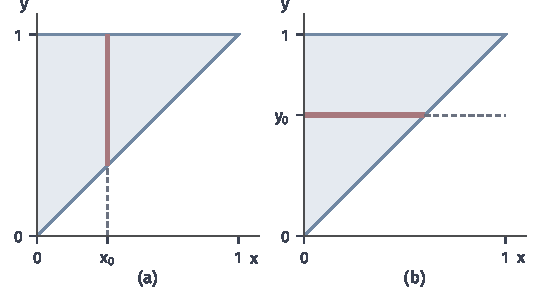
\includegraphics[width=92mm]{figures/04-spaces-measures-and-geometry/02-measure/matplotlib/integ-section-swap/figure.pdf}
  \caption{三角形$T=\{0\leq x\leq y\leq1\}$的两种截面。(a)固定$x=x_0$，红色线段是$y\in[x_0,1]$。(b)固定$y=y_0$，红色线段是$x\in[0,y_0]$，虚线部分不在$T$内。}
  \label{fig:integ-section-swap}
\end{BookInlineFigure}

\paragraph{完备化下的Tonelli定理}
若$f$只对完备化的乘积测度可测，截面函数可能不可测，结论要改成“几乎所有参数”。设$\mu,\nu$完备且$\sigma$有限，$f\geq0$对$\mu\otimes\nu$的完备化可测。

第一步找一个可测的替身。存在$\mathcal A\otimes\mathcal B$可测的$g\geq0$与$\mu\otimes\nu$零测集$N\in\mathcal A\otimes\mathcal B$，使$f=g$在$N$外成立：对指示函数，这就是完备化的定义（可测集等于乘积可测集并上零测集的子集），再经简单函数的递增逼近推广到一般的$f$。

第二步把零测的影响限制在参数上。由式~\eqref{eq:integ-product-sections}，$\int\nu(N_x)\,\mathrm d\mu=0$，所以对几乎每个$x$，$N_x$是$\nu$零测集。在这些$x$处，$f_x$与可测的$g_x$只在零测集上不同，由$\nu$的完备性可测，且积分相同。

对$g$用Tonelli定理，就得到式~\eqref{eq:integ-tonelli}，只是内层积分只对几乎每个$x$有定义，在例外的零测集上可以任意取值。$\mathbb R^d$上Lebesgue可测函数的累次积分正是这种情形。

\paragraph{$\sigma$有限条件}
$\sigma$有限条件不能省去。在$X=Y=[0,1]$上取$\mu$为Lebesgue测度，$\nu$为以全部Borel集为可测范围的计数测度，它不是$\sigma$有限的。对角线$D=\{(x,x):x\in[0,1]\}$是闭集，属于$\mathcal B([0,1])\otimes\mathcal B([0,1])$。

每个$x$截面$D_x=\{x\}$的计数为$1$，每个$y$截面$D^y=\{y\}$的Lebesgue测度为$0$，于是
\[
 \int_X\nu(D_x)\,\mathrm d\mu(x)=1,\qquad \int_Y\mu(D^y)\,\mathrm d\nu(y)=0 .
\]
两种次序不相等，式~\eqref{eq:integ-product-sections}失效。乘积测度构造中的唯一性论证正是在这里失去了依据：计数测度没有有限质量的覆盖片。

\paragraph{非负双重级数}
取两个$\mathbb N$上的计数测度，非负函数$a(m,n)=a_{m,n}$对乘积$\sigma$代数$\mathcal P(\mathbb N\times\mathbb N)$可测，乘积测度是$\mathbb N\times\mathbb N$上的计数测度。Tonelli定理给出
\[
 \sum_m\sum_na_{m,n}=\sum_n\sum_ma_{m,n},
\]
两边可以为$+\infty$：非负双重级数总可以交换求和次序。下一小节将看到，有正有负的双重级数并非如此。

\subsection{Fubini定理}
\label{sec:integ-fubini}

\paragraph{绝对可积函数的换序}
对取正负值或复值的函数，正负贡献的抵消可能依赖求和或积分的次序。解决办法是先对$\lvert f\rvert$用Tonelli定理核对绝对可积性，有了这一保证，再把$f$拆成正负部分或实部虚部，分别使用Tonelli定理。

\begin{theorem}[Fubini定理]
\label{thm:integ-fubini}
设$\mu,\nu$都是$\sigma$有限测度，$f$是$X\times Y$上$\mathcal A\otimes\mathcal B$可测的实值或复值函数，且
\begin{equation}
 \int_X\Bigl(\int_Y\lvert f(x,y)\rvert\,\mathrm d\nu(y)\Bigr)\mathrm d\mu(x)<+\infty .
 \label{eq:integ-fubini-condition}
\end{equation}
则$f$关于$\mu\otimes\nu$可积，并且：
\begin{enumerate}
 \item 对$\mu$-几乎每个$x$，$f_x$关于$\nu$可积；对$\nu$-几乎每个$y$，$f^y$关于$\mu$可积。
 \item 令$F(x)=\int_Yf_x\,\mathrm d\nu$，在$f_x$不可积的例外集上令$F(x)=0$，则$F$关于$\mu$可积；对$y$同样定义的$G$关于$\nu$可积。
 \item 三种累计相等：
 \begin{equation}
  \int_{X\times Y}f\,\mathrm d(\mu\otimes\nu)=\int_XF\,\mathrm d\mu=\int_YG\,\mathrm d\nu .
  \label{eq:integ-fubini}
 \end{equation}
\end{enumerate}
\end{theorem}

\begin{proof}
对$\lvert f\rvert$用Tonelli定理，式~\eqref{eq:integ-fubini-condition}的累次积分等于$\lvert f\rvert$在乘积空间上的积分，所以$f$可积。

令
\[
 N=\Bigl\{x:\ \int_Y\lvert f_x\rvert\,\mathrm d\nu=+\infty\Bigr\}.
\]
由Tonelli定理，它是可测集；又$x\mapsto\int\lvert f_x\rvert$的积分有限，由引理~\ref{lem:integ-null-sets}第2条，$\mu(N)=0$。这就是第1条。

先设$f$实值。$f^+$与$f^-$都是非负可测函数，由Tonelli定理，$x\mapsto\int f^\pm_x\,\mathrm d\nu$可测，积分分别等于$\int f^\pm\,\mathrm d(\mu\otimes\nu)$，都有限。在$N$外两者都有限，所以在$N$外有
\[
 F(x)=\int_Yf^+_x\,\mathrm d\nu-\int_Yf^-_x\,\mathrm d\nu .
\]
在$N$上$F=0$，所以$F$可测。对$F$积分，去掉零测集$N$不改变积分，得到
\[
\begin{aligned}
 \int_XF\,\mathrm d\mu&=\int_{X\setminus N}\Bigl(\int_Yf^+_x\,\mathrm d\nu\Bigr)\mathrm d\mu-\int_{X\setminus N}\Bigl(\int_Yf^-_x\,\mathrm d\nu\Bigr)\mathrm d\mu\\
 &=\int f^+\,\mathrm d(\mu\otimes\nu)-\int f^-\,\mathrm d(\mu\otimes\nu).
\end{aligned}
\]
右端就是$\int f\,\mathrm d(\mu\otimes\nu)$。$y$一侧对称。复值情形对实部与虚部分别使用实值结论，二者的例外集之并仍是零测集。
\end{proof}

截面只需几乎处处可积，这是由内层积分自身的性质决定的：对某个零测的$x$集合，$f_x$可能不可积，内层积分没有定义。把这些点上的$F$统一取零，得到的是一个可测的外层被积函数，而外层积分看不见零测集上的取值。若改用完备化的乘积测度，再结合上一小节的完备化讨论，结论同样成立，只是截面可测性本身也只对几乎每个参数成立。

\paragraph{缺少绝对可积时的反例}
绝对可积的假设不能去掉。考虑$\mathbb N\times\mathbb N$上的计数测度与下面的无穷矩阵，图~\ref{fig:integ-fubini-counterexample}画出了它的左上角：
\[
 a_{i,j}=\begin{cases}1,&j=i,\\-1,&j=i+1,\\0,&\text{其他}.\end{cases}
\]

先按行累计。每一行只有$+1$与$-1$两个非零元，行和为$0$，所以
\[
 \sum_i\sum_ja_{i,j}=0 .
\]
再按列累计。第一列只有$a_{1,1}=1$，列和为$1$；第$j\geq2$列有$a_{j,j}=1$与$a_{j-1,j}=-1$，列和为$0$，所以
\[
 \sum_j\sum_ia_{i,j}=1 .
\]

\begin{BookInlineFigure}
  \centering
  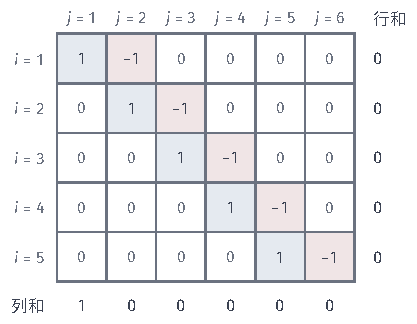
\includegraphics[width=70.672mm]{figures/04-spaces-measures-and-geometry/02-measure/tikz/integ-fubini-counterexample/figure.pdf}
  \caption{无穷矩阵$a_{i,j}$的左上角五行六列，矩阵向右下方继续。蓝色单元为$+1$，红色单元为$-1$。右侧是整行的和，下方是整列的和；第六列的$+1$位于第六行，在图外。}
  \label{fig:integ-fubini-counterexample}
\end{BookInlineFigure}

两种次序给出不同结果。原因是$\sum_{i,j}\lvert a_{i,j}\rvert=+\infty$，Fubini定理的条件不成立；每一行、每一列单独看都绝对可和，这并不够。这与有限矩阵不同：有限矩阵的两种次序总相同，因为有限和的重排不需要任何条件。

使用Fubini定理的标准步骤因此是：先对$\lvert f\rvert$任选一种方便的次序作累次积分，由Tonelli定理确认结果有限；然后才可以对$f$本身任意换序。对有界函数和有限测度，例如有界区域上的有界可测函数，第一步自动成立。
